100. $\cfrac{x^3-9x^2+20x}{x-4}\leqslant0\Leftrightarrow \cfrac{x(x^2-9x+20)}{x-4}\leqslant0\Leftrightarrow\cfrac{x(x-4)(x-5)}{x-4}\leqslant0.$ Применив метод интервалов, найдём ответ: $x\in[0;4)\cup(4;5].$
\begin{figure}[ht!]
\center{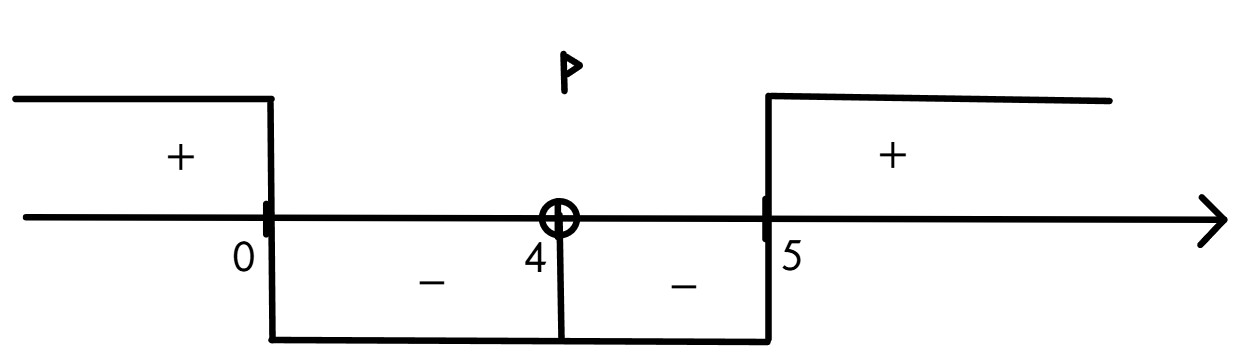
\includegraphics[scale=0.35]{int85.png}}
\end{figure}\\
